\documentclass[10pt,a4paper,final]{article}
\usepackage[pdftex]{graphicx}
\usepackage[utf8]{inputenc}
\usepackage{amsmath}
\usepackage{amsfonts}
\usepackage{amssymb}
%\usepackage{tikz}
\usepackage{empheq}

\title{Model for elastic energy of a dissociated dislocation}

\begin{document}
\section{Introduction}

The general model for the elastic energy per unit length for a mixed dislocation dissociated into two partials can be given as \cite{bacon78}:
\begin{equation}
E_D(\theta) = E_S(\theta) + E_I(\theta,\Delta) + E_F(\Delta,\gamma) \label{eqbacon}
\end{equation}
"$E_S$" is the self-energy, "$E_I$" is the interaction energy, and "$E_F$" is the fault-energy. "$\theta$" is the angle between the Burgers vector and the unit line vector, $\Delta$ is the separation between two line segments, $\gamma$ is the stacking-fault energy.\\

A general expression can be given for each energy.
\begin{subequations}
\begin{align}
E_S(\theta) & = \frac{\mu b^2}{4\pi}\left(1-\nu\cos^2\theta\right)\ln\left(\frac{R}{r_0}\right) \label{eq:ltmodel}\\
E_I(\theta) & = \frac{\mu b^2}{2\pi}\left(\alpha+\frac{\beta}{1-\nu}\right)\ln\left(\frac{R}{\Delta}\right)-\frac{\mu}{2\pi(1-\nu)}\psi \label{eq:defEi}\\
E_F & = \gamma \Delta \label{eq:defEf}
\end{align}
\end{subequations}
$r_0$ and $R$ are the inner and outer cutoff radii, respectively. $\mu$, $b$, and $\nu$ are the shear modulus, the Burgers vector of the dislocation, and the Poisson ratio.\\

Equation \ref{eq:defEi} is the interaction energy between two parallel dislocation segments separated by a vector $\vec{\Delta}$. $\alpha$, $\beta$, and $\psi$ are related to the Burgers vectors and the line direction vectors of the two dislocations. $\Delta$ is the vector pointing from one dislocation segment to the second.

$\gamma$ is the stacking-fault energy

\section{Interaction energy between two parallel in-plane dislocation segments}
The interaction energy between two parallel dislocations is defined from eq.(5-16)\cite{hirth1982theory}. It has the same form as defined in eq.(\ref{eq:defEi}). As such $\alpha$, $\beta$, and $\psi$ are defined as:
\begin{subequations}
\begin{align}
\alpha &= \left(\vec{b}_1 \cdot \hat{l}\right)\left(\vec{b}_2 \cdot \hat{l}\right) \\
\beta &= \left(\vec{b}_1 \wedge \hat{l}\right) \cdot \left(\vec{b}_2 \wedge \hat{l}\right) \\
\psi &= \frac{1}{\Delta^2}\left[\left(\vec{b}_1 \wedge \hat{l}\right) \cdot \vec{\Delta}\right]
\left[\left(\vec{b}_2 \wedge \hat{l}\right) \cdot \vec{\Delta}\right]
\end{align}
\label{eq:alphabeta}
\end{subequations}
For our case, the dislocations also exist in the same plane since they are partials. Hence $\vec{b}_i \wedge \hat{l} \perp \vec{\Delta} \Rightarrow \psi = 0$ for our model. \\ 

The form of the elastic energy is then
\begin{subequations}
\begin{align*}
E_D(\theta) &= E_S(\theta) + E_I(\theta,\Delta) + \gamma\Delta \\
 &= E_S(\theta) + \frac{\mu}{2\pi}\left(\alpha+\frac{\beta}{1-\nu}\right)\ln\frac{R}{\Delta} + \gamma\Delta
\end{align*}
\end{subequations}
Taking the partial derivative wrt $\Delta$ to find the equilibrium separation $d$
\begin{subequations}
\begin{align*}
\left.\frac{\partial E_D}{\partial\Delta}\right|_{\Delta=d} &= \frac{\mu}{2\pi}\left(\alpha+\frac{\beta}{1-\nu}\right)\frac{-1}{d} + \gamma \\
0 &= \frac{\mu}{2\pi}\left(\alpha+\frac{\beta}{1-\nu}\right)\frac{-1}{d} + \gamma \\
\end{align*}
\end{subequations} 
Which gives the relation between the equilibrium separation and the interaction energy coefficients
\begin{equation}
\gamma d = \frac{\mu}{2\pi}\left(\alpha+\frac{\beta}{1-\nu}\right) \label{eq:gammad}
\end{equation}
Replacing equation \ref{eq:gammad} in equation \ref{eqbacon} we get the general form
\begin{equation}
\boxed{
E_D(\theta) = E_S(\theta+\phi) + E_S(\theta-\phi) + \gamma d \ln\frac{R}{d} + \gamma d} \label{eq:finalED}
\end{equation}

%%%%%%%%%%%%%%%%%%%%%%%%%%%% Shockley dislocation
\section{Shockley dislocation ($\theta, \phi=\pm\pi/6$)}
\begin{figure}[hbtp]
\centering
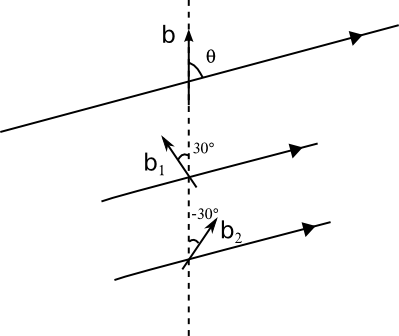
\includegraphics[scale=1]{png/shockley_schema.png}
\caption{Representation of a Shockley pair}
\end{figure}

\subsection{Self-energy}
Using equation (\ref{eq:ltmodel}) we can show that the self-energy for a pair of Shockley partials is given as
\begin{equation}
E_S\left(\theta+\frac{\pi}{6}\right) + E_S\left(\theta-\frac{\pi}{6}\right) \cong 2 - \nu\cos^2\left(\theta+\frac{\pi}{6}\right) - \nu\cos^2\left(\theta-\frac{\pi}{6}\right) \label{eq:self1shoc}
\end{equation}

Using the identity: 
\begin{equation}
\cos^2(A+B) + \cos^2(A-B) = 2(\cos^2A\cos^2B + \sin^2A\sin^2B) \label{eqcosplus}
\end{equation}

And letting $A = \theta, B = \pi/6$ we get
\begin{subequations}
\begin{align*}
\cos^2\left(\theta+\frac{\pi}{6}\right) + \cos^2\left(\theta-\frac{\pi}{6}\right) &= 
2\left(\frac{3}{4}\cos^2\theta + \frac{1}{4}\sin^2\theta \right) \\
&= \frac{1}{2}(3\cos^2\theta + \sin^2\theta) \\
&= \frac{1}{2}(1+2\cos^2\theta)
\end{align*}
\end{subequations}

Replacing in equation \ref{eq:self1shoc} gives:
\begin{equation}
\begin{split}
E_S\left(\theta+\frac{\pi}{6}\right) + E_S\left(\theta-\frac{\pi}{6}\right) &=
\frac{\mu b^2}{4\pi}\ln\left(\frac{R}{r_0}\right)\frac{1}{1-\nu}\left[2-\frac{\nu}{2}(1+2\cos^2\theta)\right] \\
&=\frac{\mu b^2}{8\pi}(4-\nu-2\nu\cos^2\theta)\ln\frac{R}{r_0} \label{eq:e_self_shockley}
\end{split}
\end{equation}

\subsection{Interaction energy}
Hirth \cite{hirth1982theory}(eq.10-15) defines the equilibrium separation between two Shockley partials as:
\begin{equation}
\gamma_B d_B = \frac{\mu b^2}{8\pi}\frac{2-\nu}{1-\nu}\left(1-\frac{2\nu\cos2\theta}{2-\nu}\right)
\label{eq:hirth1015}
\end{equation}

\subsection{Full expression}
Replacing equations \ref{eq:hirth1015} and \ref{eq:e_self_shockley} in equation \ref{eq:finalED} we get the elastic energy of a pair of Shockley partial dislocations
\begin{equation}
\begin{split}
E_D^B(\theta,\nu,\gamma) &= \frac{\mu b^2}{8\pi}\frac{4-\nu-2\cos^2\theta}{1-\nu}\ln\frac{R}{r_0} \\ 
&+\frac{\mu b^2}{8\pi}\left(1-\frac{2\nu\cos2\theta}{2-\nu}\right)\left(\ln\frac{R}{d_B} + 1 \right)
\end{split}
\label{eq:EDshoc}
\end{equation}
where $d_B$ is defined in equation \ref{eq:hirth1015}.

%%%%%%%%%%%%%%%%%%%% Prismatic pair
\section{Prismatic dislocation ($\theta, \phi= 0)$}
\begin{figure}[hbtp]
\centering
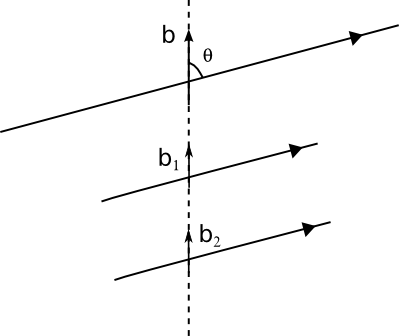
\includegraphics[scale=1]{png/prism_schema.png}
\caption{Representation of a prismatic pair}
\end{figure}
\subsection{Self-energy}
The self energy of a pair of dislocations with equal Burgers vectors ($\phi=0$) is just double that for a single
\begin{equation}
E_S(\theta) = 2\cdot\frac{\mu b^2}{4\pi}\frac{1-\nu\cos^2\theta}{1-\nu}\ln\frac{R}{r_0} \label{eq:selfprism}
\end{equation}

\subsection{Interaction energy}
There is no equation in \cite{hirth1982theory} similar to that of \ref{eq:hirth1015}, so we will derive it here.
The equilibrium separation between the pair of dislocations in the prismatic plane can be obtained from equation \ref{eq:alphabeta}

\begin{subequations}
\begin{align*}
\alpha &= b^2\cos^2\theta \\
\beta &= b^2\sin^2\theta
\end{align*}
Replacing in equation \ref{eq:gammad} gives
\begin{align*}
\gamma d &= \frac{\mu b^2}{2\pi}\left(\cos^2\theta+\frac{\sin^2\theta}{1-\nu}\right) \\
&= \frac{\mu b^2}{2\pi}\frac{1}{1-\nu}(\cos^2\theta -\nu\cos^2\theta +\sin^2\theta ) \\
&= \frac{\mu b^2}{2\pi}\frac{1}{1-\nu}(1 - \nu\cos^2\theta) \\
&= \frac{\mu b^2}{2\pi}\frac{1}{1-\nu}\left(1 - \nu\frac{\cos2\theta+1}{2}\right) \\
&= \frac{\mu b^2}{4\pi}\frac{1}{1-\nu}(2 - \nu\cos2\theta - \nu) \\
\end{align*}
And we get
\begin{equation}
\gamma_Pd_P = \frac{\mu b^2}{4\pi}\frac{2-\nu}{1-\nu}\left(1 - \frac{\nu\cos2\theta}{2-\nu}\right) \label{eq:gdprism}
\end{equation}
\end{subequations}
which is quite similar to equation \ref{eq:hirth1015} up to the constant inside the paranthases. 

\subsection{Full expression}
If we combine equations \ref{eq:gdprism} and \ref{eq:selfprism} we get
\begin{equation}
\begin{split}
E_D^P(\theta, \nu, \gamma) &=  \frac{\mu b^2}{4\pi}\frac{2}{1-\nu}(1-\nu\cos^2\theta)\ln\frac{R}{r_0} \\
&+\frac{\mu b^2}{4\pi}\frac{2-\nu}{1-\nu}\left(1-\frac{\nu\cos2\theta}{2-\nu}\right)\left(\ln\frac{R}{d_P} + 1\right)
\end{split}
\label{eq:EDprism}
\end{equation}
where $d_P$ is defined in equation \ref{eq:gdprism}.

\section{Implementation for the case of Zr}
We will take $E_0 = [\mu a^2/\pi] = [J/m]$ as units of energy and $a$ as units of distance. This allows us to define the dimensionless stacking-fault energies $\gamma'$ as 
\begin{equation}
\gamma' = \frac{\gamma}{E_0/a} = \frac{\gamma\pi}{\mu a} \label{eq:dimgamma} 
\end{equation}
We use the parameters $\mu=131~\text{GPa}$, $a=3.232~\AA$ $\gamma_P=135 ~\text{mJ/m}^2$, $\gamma_B = 198 ~\text{mJ/m}^2$ to define the prismatic and basal stacking fault-energies for zirconium
\begin{equation}
\begin{split}
\gamma_P' &= 0.000100 \\
\gamma_B' &= 0.000147
\end{split}
\label{eq:gammaszr}
\end{equation}\\

For the radii let $r_0=a$ and let $R=10^nr_0$. We also specify $d = d'.a$. This choice of parameters allows to identify the dimensionless value $d'$ and gives the following useful approximations to the natural logarithm:
\begin{equation}
\begin{split}
\ln\frac{R}{r_0} &= \ln\frac{a~10^n}{a} = \ln10^n = 2.3n \\
\ln\frac{R}{d} &= \ln\frac{10^na}{d'~a} = \ln10^n - \ln(d') = 2.3n - \ln(d')
\end{split}
\label{eq:lns}
\end{equation}

Without any loss in generality we let $n=3$ and using equations \ref{eq:lns}, \ref{eq:gammaszr}, \ref{eq:EDprism}, and \ref{eq:EDshoc} we show in figure \ref{fig:zr} the elastic energy of a dissociated dislocation in the basal plane as a function of $\theta$ and we compare with that of a dissociated dislocation in the prismatic plane.\\

We note that the screw dislocation ($\theta=0$) in the prismatic plane (green curve) has the lowest energy. The energy difference between the screw dislocation in the basal and the prismatic plane is roughly $\Delta_{PB}(\theta=0) = 504 ~\frac{\mu a^2}{\pi}$. Using the same values for the parameters of zirconium listed above $\mu$ and $a$ we get $\Delta_{PB}(\theta=0) = 6753.6~\text{J/m}$

\begin{figure}[htbp]
\centering
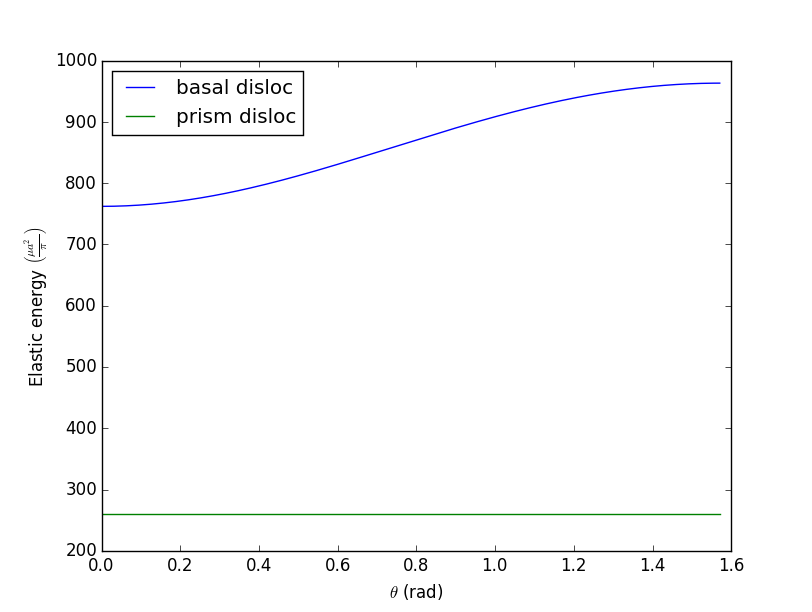
\includegraphics[scale=0.7]{png/zr_basal_prism}
\caption{Elastic energy as a function of dislocation character. Case of zirconium. $\gamma_P' = 0.000100, \gamma_B' = 0.000147, \nu=1/3$}
\label{fig:zr}
\end{figure}

\pagebreak
\bibliography{bacon78.bib,hirth82}
\bibliographystyle{plain}
\end{document}



